\section{Vorgehensweise}\label{sec:vorgehensweise}

\subsection{Projektplan}\label{subsec:projektplan}

\subsubsection*{Übersicht}
\begin{figure}[h]
    \label{fig:projectPlan}
    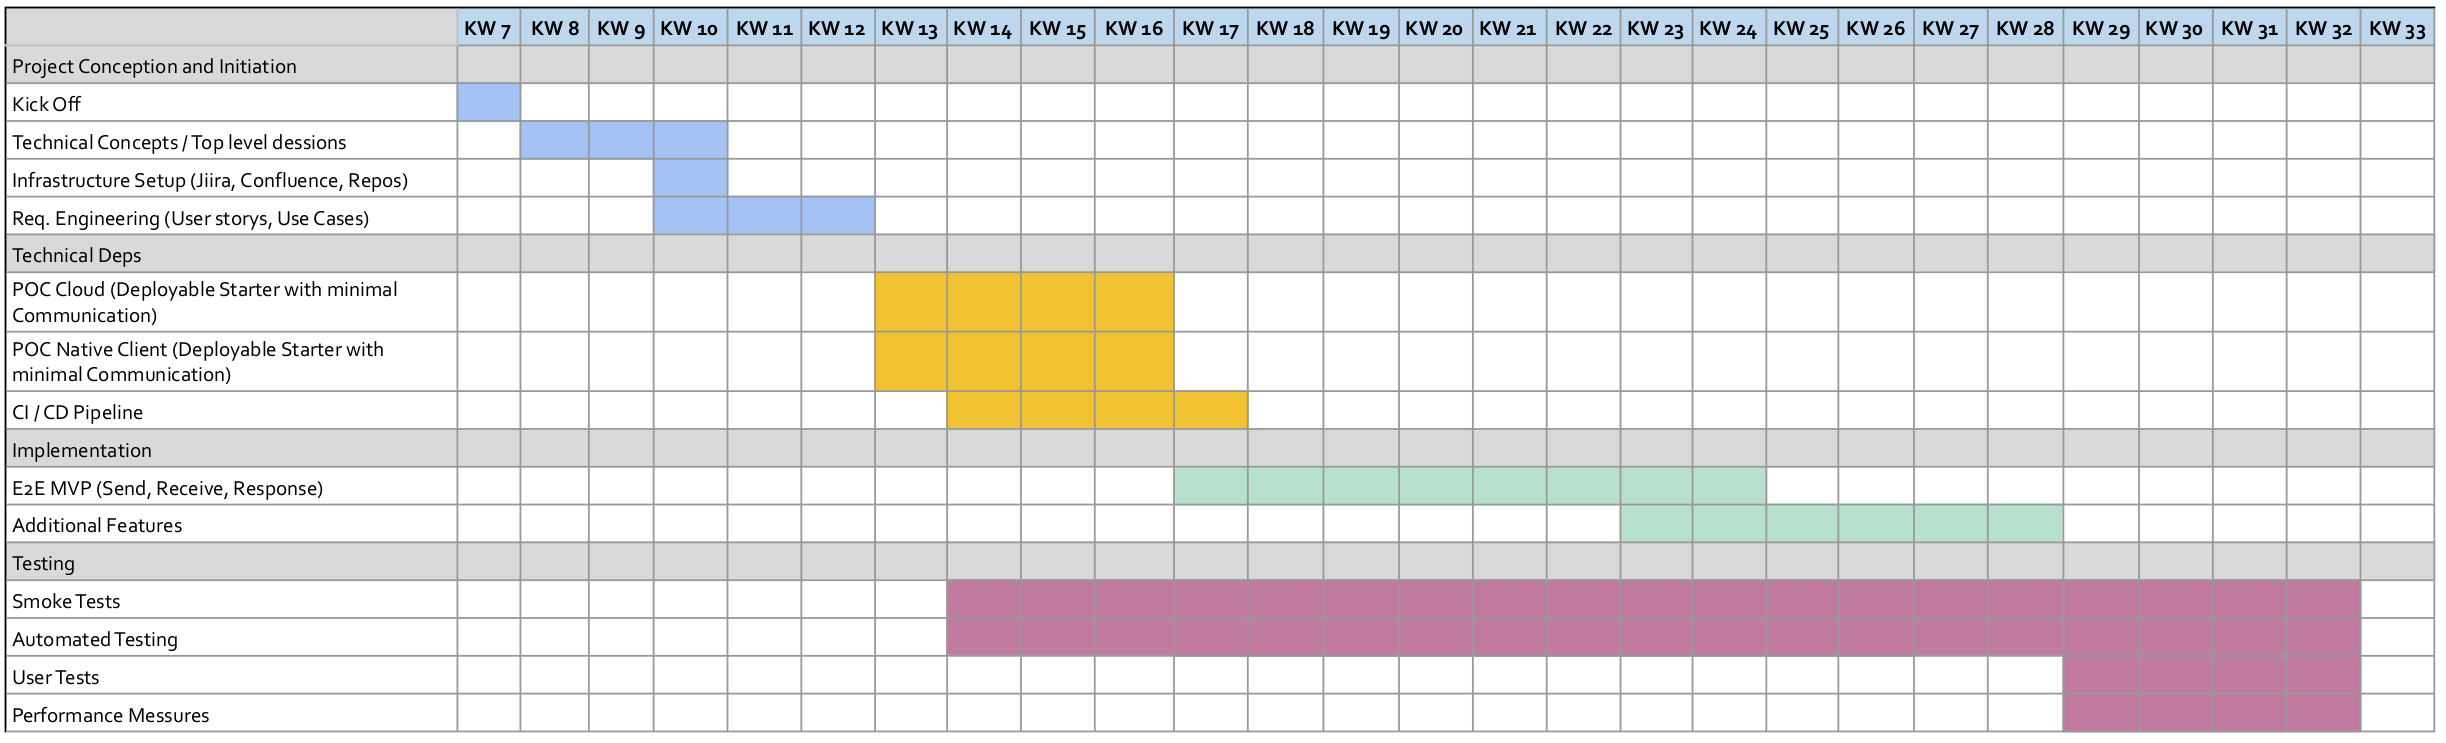
\includegraphics[width=\linewidth]{graphics/Projectplanning}\caption[Projektplan]{Projektplan}
\end{figure}

Das Projekt Cloudbasiertes Praxisrufsystem soll in vier Phasen umgesetzt werden.
Wobei sich diese Phasen teilweise überschneiden.

In der ersten Phase (KW7-KW13) wird die organisatorische Infrastruktur für das Projekt aufgebaut.
Es werden Grobkonzepte für das umzusetzende System erfasst.
Dazu werden Technologien evaluiert, die zur Umsetzung verwendet werden können und
die wichtigsten Ziele des Projektes als Milestones festgehalten.

In der zweiten Phase (KW13-KW17) wird ein Proof Of Concept erstellt.
Dieser soll die gültigkeit der Resultate aus Phase 1 verifizieren.
Wenn nötig werden hier Anpassungen an den gewählten Technologien und erstellten Grobkonzepten gemacht.
Die Architektur und das Konzept werden weiter verfeinert und erste Anforderungen werden konkretisiert.

In der dritten Phase (KW17-KW38) wird das Projekt umgesetzt.
Zur Umsetzung gehört dabei, laufend die als nächstes umzusetzenden Anforderungen im Detail zu definieren und die Konzepte dafür zu erweitern.

Die vierte Phase (KW14-KW32) läuft parallel zur Dritten und beschäftigt sich mit dem Testen des Systems.
Automatisierte Unit und Smoke Tests sollen während der ganzen Projektdauer für die entwickelten Komponenten gemacht werden.
Zum Ende des Projekts soll das System zudem mit dem Benutzer getestet werden und auf Performance geprüft werden.

\clearpage
\subsection{Milestones}

In der Anfangsphase des Projektes wurden folgende Milestones definiert:

\begin{table}[h]
    \centering
    \begin{tabular}{|l|p{15cm}|}
        \hline
        \textbf{Id} & \textbf{Beschreibung}                                                                                                                                                                                         \\
        \hline
        M01         & Proof Of Concept - Setup. Ein Mobile Client kann auf IOS installiert werden und mit einem Backendservice kommunizieren. \\
        \hline
        M02         & Proof Of Concept - Messaging. Ein Mobile Client kann Benachrichtigungen empfangen und Push-Benachrichtigungen anzeigen. \\
        \hline
        M03         & Versenden mit Registration. Mobile Clients können sich beim Praxisrufsystem registrieren und Benachrichtungen empfangen. Alle registrierten Clients erhalten alle Benachrichtigungen. \\
        \hline
        M04         & Benachrichtigungen konfigurierbar. Der Mobile Client lädt seine Konfiguration vom Backend und zeigt dynamisch konfigurierte Buttons an über die Benachrichtigungen versendet werden.\\
        \hline
        M05         & Setup Wizard für Konfiguration. Ein Administrator kann das System über eine Benutzeroberfläche konfigurieren.  \\
        \hline
        M06         & 1:N Versenden Konfigurierbar. Es kann konfiguriert werden, welcher Client sich für welche Benachrichtigungen interessiert. Alle Clients erhalten nur für sie relevante Benachrichtigungen.  \\
        \hline
        M07         & Voice to Speech. Empfangene Benachrichtigungen können dem Benutzer vorgelesen werden. \\
        \hline
        M08         & Raspberry Pi Anbindung. Benachrichtigungen können über ein Raspberry Pi mit angeschlossenem Button versendet werden. \\
        \hline
        M09         & Sprachkommunikation 1:1. Der Mobile Client unterstützt direkte Anrufe zwischen zwei Geräten. \\
        \hline
        M10         & Sprachkommunikation 1:n. Der Mobile Client unterstützt Gruppenanrufe mit mehreren Geräten gleichzeitig. \\
        \hline
    \end{tabular}\label{tab:milestones}
\end{table}
\clearpage


